\chap{Introduction}

% \begin{flushright}
%   \textit{Everything should be made as simple as possible, but not simpler.}\\
%   {---Albert Einstein}
% \end{flushright}
% As you know from teaching introductory statistics, 30 is infinity. -- Andrew Gelman
% The best thing about being a statistician is that you get to play in everyone's backyard. --- John Tukey

% \epigraph{\itshape
%   As you know from teaching introductory statistics, 30 is infinity.
% }{
%   ---Andrew Gelman
% }
\epigraph{\itshape
  If we have data, let’s look at data. If all we have are opinions, let’s go with mine.
}{
  ---Jim Barksdale
}

\section{Background}

With modern advances in science and technology, statistical models and the data on which they are fit are becoming increasingly complex. Datasets are expanding in size, often both in terms of their numbers of variables (features) as well as observations. In some fields, this growth in complexity has been paralleled with more effective methods with which to collect observations, as in crowd science and recommender systems. But in other areas, collecting data still amounts to a costly endeavor. In bioinformatics, for example, ethical concerns and rising requirements on the quality of data have only served to \emph{raise} the costs of data collection. As a result, data collected in these fields is becoming \emph{wider}: the ratio between the number of variables (features) and the number of observations is increasing~(\Cref{tab:types-of-data}).

\begin{table}[htbp]
  \caption{Tall and wide data. Each row is an observation, for instance the measurement on a person in a study, and each column a feature, which represents all the measurements on a variable for all the observations.}
  \label{tab:types-of-data}
  \begin{subtable}{.44\linewidth}\centering
    \caption{Tall data}
    {\begin{tabular}{S[table-format=1.0]S[table-format=1.2]S[table-format=1.0]}
        \toprule
        {Feature 1} & {Feature 2} & {Feature 3} \\
        \midrule
        0           & 0.32        & 1           \\
        1           & -1.2        & -1          \\
        $\vdots$    & $\vdots$    & $\vdots$    \\
        \bottomrule
      \end{tabular}}
  \end{subtable}\hfill%
  \begin{subtable}{.51\linewidth}\centering
    \caption{Wide data}
    {\begin{tabular}{S[table-format=1.0]S[table-format=1.2]S[table-format=1.0]c}
        \toprule
        {Feature 1} & {Feature 2} & {Feature 3} & $\cdots$ \\
        \midrule
        0           & 0.32        & 1           & $\cdots$ \\
        1           & -1.2        & -1          & $\cdots$ \\
        \bottomrule
      \end{tabular}}
  \end{subtable}%
\end{table}

The growth in the number of observations (taller data) is mostly a luxury problem since more observations typically mean more accurate models. But an expansion in the number of features (wider data) is a more delicate issue. The problem is that if all the features that we have collected are important then we are out of luck as far as understanding our data goes. Instead, we have to more or less hope that there is a \emph{sparse} representation of our data that, with some acceptable loss of information, allows us to make sense of the problem we are studying.

We can call this hope the \emph{sparsity assumption}, which can be motivated through the \emph{bet-on-sparsity} \emph{principle}: assume that the underlying signal is sparse~(\Cref{fig:sparse-signal}) and use a sparse method to model it. If the assumption is correct, then our method has a chance of doing well. But if the assumption is incorrect, then our method will not work---but no other method would~\parencite{hastie2009}. Thankfully, many problems in the real world exhibit this type of sparsity.

\begin{figure}[pb]
  \centering
  \includegraphics[]{figures/sparse-signal.pdf}
  \caption{%
    A relatively sparse signal. The plot shows correlations between the response vector \(\vec{y}\) and each feature in the \data{madelon} dataset~\parencite{guyon2004}. Correlations above 0.1 have been colored in black, the rest in gray.
  }
  \label{fig:sparse-signal}
\end{figure}

The success of neural networks and other complex models that model high-dimensional data well yet do not enforce sparsity does raise questions as to the validity of this principle. But in our setting, which, loosely speaking, is \emph{explainable} methods for regression, it still bears relevance.

Technically speaking, we are interested in datasets that are made up of a \(n \times p\) matrix of features \(\mat{X}\) and a response vector of length \(n\), \(\vec{y}\):
\[
  \mat{X} = \begin{bmatrix}
    0       & 0.32    & \cdots & x_{1,p} \\
    1       & -1.2    & \cdots & x_{2,p} \\
    \vdots  & \vdots  & \ddots & \vdots  \\
    x_{n,1} & x_{n,2} & \cdots & x_{n,p} \\
  \end{bmatrix},\qquad
  \vec{y} = \begin{bmatrix}0.2 \\ -0.9 \\ \vdots \\ y_n\end{bmatrix},
\]
where we have inserted some arbitrary values for the sake of illustration. The data presented in \Cref{tab:types-of-data} corresponds to \(\mat{X}\) here (each row is an observation, each column a feature).

In the simplest case, we assume that \(\vec{y}\) is a linear combination of the features in \(\mat{X}\) plus some noise (\(\vec{\varepsilon)}\), for instance measurement noise, which we write mathematically as
\[
  \vec{y} = \mat{X}\vec{\beta} + \beta_0 + \vec{\varepsilon},
\]
where \(\vec{\beta}\) is a vector of coefficients and \(\beta_0\) the \emph{intercept}. In this representation of the data, the coefficients \(\vec{\beta}\) are the parameters that we are interested in estimating and represent the effect each feature has on the response vector \(\vec{y}\).
Assuming that this is in fact the true relationship between \(\vec{\beta}\), \(\mat{X}\), and \(\vec{y}\), a natural choice of model to fit this data with is \emph{linear regression}.\footnote{In general, we also need additional assumptions on the noise term \(\vec{\varepsilon}\).}

In the presence of noise, however, there generally exists no \(\beta_0\) and \(\vec{\beta}\) that will fit the data perfectly, and we must therefore accept that the linear regression model is only an approximation. The natural follow-up question is then: what \emph{is} a good approximation? To answer this question, we need to define some measure of error. The most common measure, at least as far as linear regression models go, is the sum of squared errors between the predicted response vector
\[
  \hat{\vec{y}} = \mat{X}\hat{\vec{\beta}}
\]
and the true response vector \(\vec{y}\), that is,
\[
  \lVert \vec{y} - \hat{\vec{y}}\rVert^2_2 = \sum_{i=1}^n (y_i - \hat{y}_i)^2.
\]
The smaller this measure---the better the fit, which means that finding a vector \(\vec{\beta}\) that minimizes this error can be posed as the following optimization problem:
\begin{problem}
\label{pb:ols}
\begin{aligned}
   & \text{minimize} &  & \frac{1}{2} \lVert \vec{y} - \mat{X}\vec{\beta}\rVert^2_2.
\end{aligned}
\end{problem}
We let \(\vec{\beta}^*\) to be the solution to this problem---the optimum, and will use \(\hat{\vec{\beta}}\) to refer to the estimate that we obtain from some algorithm. Generally, we will assume that the algorithm has converged to the optimum so that \smash{\(\vec{\beta}^* = \hat{\vec{\beta}}\)}, but in actuality we almost always have some amount of \emph{suboptimality} so that \smash{\(|\hat{\vec{\beta}} - \vec{\beta}| > 0\)}. The factor \(1/2\) in \Cref{pb:ols} is included for convenience, for reasons that will become clear later on.

Solving \Cref{pb:ols} is equivalent to fitting the ordinary least-squares (OLS) regression model, which, for a simple case of a single feature, we have illustrated in \Cref{fig:ols}. Picking a different measure of error would lead to a different method (and often a different linear regression line), but in this thesis we will focus on the method of least squares.

\begin{figure}
  \centering
  \subcaptionbox{%
    The slope of the orange line is \(\beta\). The point where the line intersects the y-axis is the intercept \(\beta_0\).
  }{\includegraphics[]{figures/ols-clean.pdf}}\hspace*{1cm}%
  \subcaptionbox{%
    The dotted lines are the residuals and the grey squares are the squared errors.
    The orange line is that which minimizes the total surface of all of these squares summed together.
  }{\includegraphics[]{figures/ols-squares.pdf}}
  \caption{%
    Simple ordinary least-squares linear regression for a one-feature problem}
  \label{fig:ols}
\end{figure}

If we have many more observations than features (\(n \gg p\)), then our linear regression model might stand a decent chance of recovering the true model (coefficients). But if the tables were turned and the features instead outnumbered the observations (\(p \gg n\)), the model would in fact break down.

The problem is that our linear regression model will be able to fit our particular dataset perfectly but typically not generalize well to new data, even if it comes from the same underlying data-generating mechanism. This is called \emph{overfitting} and it happens because we have more parameters (regression coefficients) than unknowns (observations). This means that there are now many different regression models that will fit the data equally well and that the solution, therefore, is not unique. In \Cref{fig:overfitting}, we illustrate what overfitting looks like for the linear regression model in one and two parameters.

\begin{figure}
  \centering
  \subcaptionbox{%
    With one feature, the simple ordinary least-squares regression line fits the data perfectly.
  }{\includegraphics[]{figures/overfit-2d.pdf}}\hfill%
  \subcaptionbox{%
    With two features, an infinite number of regression planes fits the data perfectly.
  }{\includegraphics[]{figures/overfit-3d.pdf}}
  \caption{%
    A linear regression problem with two observations. The example is of course artifical, but demonstrating overfitting in more dimensions than this would require more than the faculties of our limited human minds are capable of.
  }
  \label{fig:overfitting}
\end{figure}

% It is also a case of the curse of dimensionality, in the sense that, as we increase the dimensions of our feature space, our observations start to effectively grow further, and further apart, and occupy less and less of the available space.

In principle, the problem of overfitting in linear regression is the same as that in polynomial regression: as we increase the number of parameters (degree of the polynomial in this case), the model eventually becomes too flexible and overfits~(\Cref{fig:polyfit}).
Note that in this example overfitting occurs even when the number of parameters is smaller than the number of observations. This is the case with linear regression too, for which the problem  may occur in cases when \(n\) is larger than \(p\).

\begin{figure}
  \centering
  \includegraphics[]{figures/polyfit.pdf}
  \caption{%
    Polynomial regression for a one-feature problem.
    The data is generated from the simple linear model \( = 2x_i + \varepsilon_i\),
    where \(\varepsilon \sim \normal(0, 0.5^2)\) identically and independently.
    The line fits the data increasingly well as the degree of the polynomial increases, but when new data arrives (the blue points), we see that the model generalizes poorly.
  }
  \label{fig:polyfit}
\end{figure}

One way to deal with overfitting is to decrease the complexity of the model by restricting the parameters in some way, for instance by allowing only a subset of the regression coefficients to be non-zero---in other words, make the model sparse. This procedure is called \emph{regularization}.

\section{Regularization}

When we regularize a model, we introduce a budget on \(\vec{\beta}\), allowing only some of its elements to be non-zero or restricting the values they can take.
The simplest type of regularization is called \emph{best-subset selection}, in which we simply limit the number of coefficients we allow to be non-zero to a constant \(k\), which is equivalent to selecting \(k\) of the features in \(\mat{X}\). We call the indices of the selected features the model's \emph{support}. If features one and three are selected, for instance, then the support is \(\{1,3\}\). If all of the features are in the model, then the support is \(\{1,2,\dots,p\}\) (as in the case of OLS regression). Finally, if no features are selected, then the support is the empty set (\(\emptyset\)).

In best-subset selection, we examine all \(\binom{p}{k}\) possible combinations of features and pick the combination that fits our data best. Formally, the method can be posed as the following optimization problem:
\[
  \begin{aligned}
     & \text{minimize}   &  & \frac{1}{2} \lVert \vec{y} - \mat{X}\vec{\beta}\rVert^2_2, \\
     & \text{subject to} &  & \lVert \vec{\beta} \rVert_0 \leq k,
  \end{aligned}
\]
where \(\lVert \cdot \rVert_0\) is the \(\ell_0\) norm:\footnote{Technically speaking, the \(\ell_0\) norm is not actually a true norm.} the number of non-zero elements in vector.

In other words, if \(p = 3\) and \(k = 2\), for instance, the following models would satisfy our constraints:
\[
  \vec{\beta} = \begin{bmatrix}0 \\ 0 \\ 0\end{bmatrix},\qquad \vec{\beta} = \begin{bmatrix}1 \\ 2 \\ 0\end{bmatrix},\qquad \text{and} \qquad \vec{\beta} = \begin{bmatrix}0 \\ 0 \\ 1\end{bmatrix}.
\]
But the following model would not:
\[
  \vec{\beta} = \begin{bmatrix}1 \\ 2 \\ 3\end{bmatrix}.
\]

% There are two problems with this method. The first is that the method involves no shrinkage, which \textcite{stein1956,james1961} in pivotal work asserted was necessary for good performance.

The primary problem with this method is that it is computationally infeasible when \(p\) is large since the number of possible models grows exponentially with \(p\). With \(p = 100\) and \(k = k\), for instance, there are
\[
  \binom{100}{5} = \num{75287520}
\]
possible models to consider. And this problem is further exacerbated by the fact that we typically has to consider a variety of values for \(k\).

In an interesting turn of events, however, \textcite{bertsimas2016} has shown that the best subset selection problem can actually be written as a mixed-integer optimization problem. This enables the use of modern optimization software, which can then handle best subset problems of dimensions that previously were thought unattainable. Yet, although this result has offered a considerable improvement in run-time performance for the algorithm, it is still the case that it struggles in high dimensions. Solving a problem with \(n=500\) and \(p=100\) for \(k \in \{1,2,\dots,50\}\), for instance, still comes down to a hefty 76.8 hours of computation~\parencite{hastie2020}. In contrast, the time taken to fit the model that we will consider next, the lasso, amounts to 0.014 seconds for the equivalent problem.

\subsection{The Lasso}

One solution to the complexity problem of best-subset selection is to relax the constraint to one that makes the problem easier to solve, yet still retains the sparsity-enforcing property of the \(\ell_0\) norm. A natural candidate for this is the \(\ell_1\) norm, which leads to the following problem,
\begin{problem}
\label{pb:lasso}
\begin{aligned}
   & \text{minimize}   &  & \frac{1}{2} \lVert \vec{y} - \mat{X}\vec{\beta}\rVert^2_2, \\
   & \text{subject to} &  & \lVert \vec{\beta} \rVert_1 \leq t,
\end{aligned}
\end{problem}
where all we did was replace the \(\ell_0\) norm with the \(\ell_1\) norm,
\[\lVert \vec{\beta}\rVert_1 = \sum_{j=1}^p |\beta_j|\]
As a consequence, we have replaced the integer-valued \(k\) with a real-valued (but positive) \(t\). This problem is known as \(\ell_1\)-regularized regression or, more commonly, as the \emph{lasso}\footnote{The lasso is sometimes written as the acronym LASSO for \emph{least absolute shrinkage and selection operator}, but we will stick with the lower-case version here, which the authors themselves use in their recent work.}. The lasso was introduced to the statistics community by \textcite{tibshirani1996} but actually stems from much earlier research done in the field of signal processing by \textcite{santosa1986}. \textcite{donoho1994,donoho1995} subsequently introduced the concept of the \emph{basis pursuit} problem, which is closely related to the lasso, and developed much of the theoretical framework for the lasso.

If you have encountered the lasso previously, it is likely that you have seen it formulated as the following unconstrained optimization problem:
\[
  \begin{aligned}
     & \text{minimize} &  & \frac{1}{2} \lVert \vec{y} - \mat{X}\vec{\beta}\rVert^2_2 + \lambda \lVert \vec{\beta}\rVert_1.
  \end{aligned}
\]
In this section, however, we will prefer the constrained formulation of the problem as it is given in \Cref{pb:lasso}, which we think is intuitive and easier to understand. The two formulations are equivalent, however, and will lead to exactly the same solution for a suitable choice of \(t\) and \(\lambda\). Later, in \Cref{sec:iterative-optimization}, we will make this connection clear.

We saw previously that the \(\ell_0\) constraint in best-subset selection puts a budget on the number of features allowed in the model. The \(\ell_1\) norm, in contrast, instead puts a budget on the \emph{size} of the coefficients. This enforces not only sparsity but also shrinkage in the solution. In \Cref{fig:lasso-ball}, we have visualized how this constraint affects the solution of the least-squares objective.

\begin{figure}
  \centering
  \subcaptionbox{A sparse solution, \(\beta_1 = 0\) and \(\beta_2 = -1\).}{\includegraphics[]{figures/lasso-ball-sparse.pdf}}\hfill%
  \subcaptionbox{A dense solution, \(\beta_1 = 0.5\) and \(\beta_2 = 0.5\).}{\includegraphics[]{figures/lasso-ball-dense.pdf}}\hfill%
  \subcaptionbox{A solution in which the constraint is inactive (\(t\) is too large to affect the solution), \(\beta_1 = 0.4\) and \(\beta_2 = 0.3\).}{\includegraphics[]{figures/lasso-ball-inactive.pdf}}

  \caption{%
    The \(\ell_1\) norm ball in \(\mathbb{R}^2\) with some possible solutions indicated by \(\vec{\beta}\). The \(\ell_0\) ball (for best-subset selection) and \(k = 1\) would be lines of infinite length along both of the axes.
  }
  \label{fig:lasso-ball}
\end{figure}

There is an extensive body of work on the lasso and it has spawned a number of offshoots, such as the fused lasso~\parencite{tibshirani2005}, group lasso~\parencite{yuan2005}, adaptive lasso~\parencite{zou2006}, graphical lasso~\parencite{friedman2008}, and square-root lasso~\parencite{belloni2011}. In this thesis, however, we focus on the standard lasso.

Note, also, that the lasso is not limited to just regularized \emph{linear} regression but can in fact be used for the entire family of generalized linear models, such as logistic, Poisson, multinomial, and multivariate regression, as well as survival models such as Cox regression. The use of the \(\ell_1\)-norm penalty has also found its way into many other areas of statistics as well as the fields of signal processing and machine learning, including matrix factorization, clustering, and deep learning.

An interesting property of the lasso is that it is possible (and computationally feasible) to exactly solve the lasso problem for all possible values of \(t \in [0, \infty)\). This is called the \emph{lasso path}~(\Cref{fig:lasso-path}). It begins at \(t=0\), for which the constraint region is a point, forcing all of the coefficients to be exactly zero. Then as \(t\) increases, the constraint region grows, allowing the coefficients to enter the model and grow. The reason for why it is possible to solve for the full path is that the solution vector \(\beta\), as a function of \(t\), is linear and continuous between the values of \(t\) for which features enter or leave the model.

\begin{figure}
  \centering
  \includegraphics[]{figures/lasso-path.pdf}
  \caption{%
    The lasso path for the \data{diabetes} dataset~\parencite{efron2004}, which consists of \(n=442\) observations and \(p=10\) features. The path shows the coefficients as a function of the parameter \(t\), which controls the size of the constraint region. The path is piecewise linear with kinks occurring only when features enter or exit the model.
    At \(t = 0\), the model is completely sparse and the support is \(\emptyset\)---the empty set. At \(t/\max t = 1\), the model is the ordinary least-squares model and the support is the full set of predictors, \(\{1,2,\dots,p\}\).
  }
  \label{fig:lasso-path}
\end{figure}

One problem with the lasso, however, is that it does not deal with correlated features as intuition (at least that of the author) would suggest. If two features are correlated highly enough, for instance, the lasso will select one of them and drop the other (set its coefficient to zero).\footnote{In the case where the features are perfectly correlated, it may in fact be the optimization algorithm that decides which of them is picked.} This is not necessarily a problem for the prediction \(\hat{\vec{y}}\), but it means that the estimated coefficients no longer provide trustworthy estimates of variable (feature) importance. This effect is the result of the behavior of the \(\ell_1\) norm, which penalizes the \emph{size} of the coefficients. If two features provide the same, or nearly the same, information about the response, then the optimization problem can attain a lower value by setting one of the coefficients to zero.

This is a problem that the \emph{elastic net}---the topic of the next section---is designed to overcome.

\subsection{The Elastic Net}

The elastic net is a combination of the lasso and ridge regression,\footnote{Ridge regression is also known as Tikhonov regression; and in deep learning, \(\ell_1\)-regularization is typically called \emph{weight decay}.} which can be written as the following optimization problem:
\begin{problem}
\label{pb:elastic-net}
\begin{aligned}
   & \text{minimize}   &  & \frac{1}{2} \lVert \vec{y} - \mat{X}\vec{\beta}\rVert^2_2,                           \\
   & \text{subject to} &  & \alpha \lVert \vec{\beta} \rVert_1 + (1-\alpha) \lVert \vec{\beta}\rVert_2^2 \leq t. \\
\end{aligned}
\end{problem}
The difference compared to the lasso is that we have transformed our constraint into a linear combination of the \(\ell_1\) and squared \(\ell_2\) norms. The parameter \(\alpha\) controls the balance between these constraints. By setting \(\alpha = 1\), we turn the problem into the lasso~(\Cref{fig:elasticnet-balls-lasso}). And at \(\alpha = 0\), we instead have ridge regression~(\Cref{fig:elasticnet-balls-ridge}). Any value \(\alpha \in (0, 1)\) yields a combination of the two~(\Cref{fig:elasticnet-balls-elasticnet}).

\begin{figure}[htpb]
  \centering
  \subcaptionbox{%
    When \(\alpha = 1\), the constraint is
    the lasso (\(\ell_1\)-norm) ball. And in this case the solution is sparse.\label{fig:elasticnet-balls-lasso}
  }{\includegraphics{figures/elasticnet-balls-lasso}}\hfill%
  \subcaptionbox{%
    When \(\alpha = 0\), the constraint is the ridge (squared \(\ell_2\)-norm) ball. Here, the solution is not sparse.\label{fig:elasticnet-balls-ridge}
  }{\includegraphics{figures/elasticnet-balls-ridge}}\hfill%
  \subcaptionbox{%
    When \(\alpha \in (0, 1)\), the constraint region is a combination of the lasso and ridge balls. In this case we have \(\alpha=1/2\). Once again, the solution is sparse.\label{fig:elasticnet-balls-elasticnet}
  }{\includegraphics{figures/elasticnet-balls-elasticnet}}
  \caption{%
    The constraint regions for the elastic net for different values of \(\alpha\)
  }
\end{figure}

The elastic net was first proposed by \textcite{zou2005}. In addition to dealing with the problems encountered in using the lasso for highly correlated features, the elastic net also yields improved predictive performance in many situations. The latter fact is perhaps not so surprising given that it is a combination of methods that essentially assume different structure in the data. The lasso works well when the true signal is sparse, while ridge regression handles the situation where there are weak signals better. And since the elastic net contains both these models as special cases, in addition to any combination thereof, it naturally extends to a wider range of problems.

\subsection{SLOPE}\label{sec:slope}

Another way of dealing with the problem of correlated features is to use \emph{Sorted L-One Penalized Estimation} (SLOPE)~\parencite{bogdan2013,zeng2014,bogdan2015}. SLOPE is a generalization of both the lasso and \emph{the octagonal shrinkage and clustering algorithm for regression} (OSCAR)~\parencite{bondell2008}. It is represented by the following optimization problem:
\begin{problem}
\label{pb:slope}
\begin{aligned}
   & \text{minimize}   &  & \frac{1}{2} \lVert \vec{y} - \mat{X}\vec{\beta}\rVert^2_2, \\
   & \text{subject to} &  & \sum_{j=1}^p \lambda_j |\beta|_{(j)} \leq t,
\end{aligned}
\end{problem}
where \(\vec{\lambda}\) is a non-increasing and non-negative sequence of penalization weights and
where we define the subscript operator \((j)\) such that
\[
  |\beta|_{(1)} \geq |\beta|_{(2)} \geq \cdots \geq |\beta|_{(p)}.
\]
The left-hand side of the constraint in SLOPE is, perhaps somewhat surprisingly, actually a norm: the \emph{sorted \(\ell_1\) norm}.

One of the most salient features of SLOPE is that it clusters coefficients~\parencite{figueiredo2014,schneider2022}. This is a consequence of the sorted \(\ell_1\) norm and the choice of \(\vec{\lambda}\)---larger differences between adjacent elements increase the propensity for clustering. This property makes SLOPE well-adapted to the case when features are highly correlated, which is a situation that the lasso struggles with. In cases where the lasso might set one of the correlated features to zero, SLOPE will often instead set them to exactly the same value. This is a property that is not shared by the elastic net, which handles correlation (although not quite as delicately), but does not cluster coefficients.

But as we mentioned previously, SLOPE is actually a generalization of lasso and thus contains it as a special case~(\Cref{fig:slope-balls-lasso}), which is attained by setting all of the elements of the penalization weight vector \(\vec{\lambda}\) to the same value. On the opposite end, setting only the first element to a non-zero value and the remaining ones to zero yields the infinity norm~(\Cref{fig:slope-balls-inf}).

% TODO: consider splitting this into a 2-by-2 grid instead.
\begin{figure}[htpb]
  \centering
  \subcaptionbox{%
    When \(\lambda_1 = \lambda_1 = 1\), the constraint region is the lasso ball, \(\lVert \vec{\beta}\rVert_1\).\label{fig:slope-balls-lasso}
  }{\includegraphics{figures/slope-ball-0.pdf}}\hfill%
  \subcaptionbox{%
    Here we have \(\lambda_1 = 1\) and \(\lambda_2 = 3/4\), but no clustering.
  }{\includegraphics{figures/slope-ball-1.pdf}}\hfill%
  \subcaptionbox{%
    With \(\lambda_1 = 1\) and \(\lambda_2 = 1/4\), the solution is now clustered.
  }{\includegraphics{figures/slope-ball-2.pdf}}\hfill%
  \subcaptionbox{%
    When \(\lambda_1 = 1\) and \(\lambda_2 = 0\), the constraint is the infinity norm, \(\lVert \vec{\beta}\rVert_\infty\).\label{fig:slope-balls-inf}
  }{\includegraphics{figures/slope-ball-3.pdf}}
  \caption{%
    SLOPE balls (the sorted \(\ell_1\) norm) for various choices of the penalization weight vector \(\vec{\lambda}\). It is the kinks at the boundaries, occurring when \(|\beta_1| =|\beta_2|\), that induce clustering. The larger the difference between adjacent values in \(\vec{\lambda}\), the stronger the clustering effect becomes.
  }
  \label{fig:slope-balls}
\end{figure}

SLOPE also has other appealing properties, such as the ability to (under certain assumptions on the design) control the false discovery rate\footnote{By false discovery rate, we mean the fraction of coefficients incorrectly identified as non-zero (false discoveries) as a proportion of the total number of non-zero coefficients (discoveries).}~\parencite{bogdan2015} and recover sparsity and ordering patterns in the solution~\parencite{bogdan2022}. Another key feature is that the problem is convex, which has implications that we will come to appreciate in \Cref{sec:optimization}. This latter fact also puts SLOPE apart from other competing penalization methods such as the minimax concave penalty~(MCP)~\parencite{zhang2010} and smoothly clipped absolute deviation (SCAD)~\parencite{fan2001}.

The constraints in the lasso and elastic net are parameterized by one and two parameters, respectively: \(t\) in the case of the lasso, and \((t, \alpha)\) in the case of the elastic net. SLOPE, in contrast, is parameterized not only by \(t\) but also by the \(\vec{\lambda}\) vector, which has \(p\) elements---one for each feature. Finding an optimal setting for all of those \(p + 1\) parameters is a non-trivial task when \(p\) is large. As a result, we typically need to re-parameterize the problem. The most common form for this parameterization is the Benjamini--Hochberg sequence, which sets the penalization weights to
\[
  \lambda_i = \Phi^{-1}(1 - q_i), \qquad q_i = \frac{q i}{2p},
\]
where \(\Phi^{-1}\) is the quantile function of the standard normal distribution and \(q \in [0, 1]\). It is this choice that gives SLOPE its false discovery rate control property~\parencite{bogdan2015}. Note that if we use a linearly decreasing sequence instead, then we would recover OSCAR. And if we use a constant sequence, we recover the lasso.

This reparameterization reduces the number of parameters to just two: \((t,q)\)---the same number as the elastic net. And it means that it is tractable to find optimal settings for the parameters using the methods that we will introduce in the next section.

\subsection{Hyperparameter Optimization}

An issue that we have so far largely ignored is how to pick good values for \(t\) in the case of the lasso, \((t,\alpha)\) in the case of the elastic net, and \((t, q)\) in the case of SLOPE. We call these \emph{hyperparameters} of the problems. Under strong assumptions on our data, in particular the error term \(\vec{\varepsilon}\), it is possible to derive optimal settings of some of these hyperparameters. The problem, however, is that we typically do not know the distribution of the error term. And in high dimensions, estimating it is not easy either.

The alternative, which is the dominating procedure in practice, is to resort to hyperparameter optimization, in which we treat the problem of finding good hyperparameters as an upper-level optimization problem (on top of the optimization problem of finding \(\vec{\beta}\)). This procedure is often also called \emph{model validation}. This is most commonly done via a grid search in which we construct a grid across the hyperparameter space. In the lasso case, for instance, it is common to construct a linearly spaced sequence of \(t\) values.\footnote{If we were to use the unconstrained version of the lasso in which the model is parameterized by \(\lambda\), the sequence is typically \emph{geometrically} spaced instead.}

In the simplest case, typically called \emph{hold-out validation}, we split the dataset into a training set and a validation set. The lasso is fit for the full \(t\) sequence on the training data; in other words, we fit a full lasso path. Afterwards, we measure the model's error on the validation data and pick the \(t\) value with the best score. Often, there is also a separate test dataset that is held-out before hyperparameter optimization; at the end, this test set is used to obtain a final unbiased goodness-of-fit measure for the model selected during hyper-optimization.

A more common, although slightly more involved, method is to use \(k\)-fold cross-validation~(\Cref{fig:k-fold-cv}), which is similar to hold-out validation, except the data is iteratively split into \(k\) folds; the method is run for as many iterations. In the \(k\)th iteration, the \(k\)th fold is held out as a validation set on which an error is computed after the model has been fit on the remaining \(k-1\) folds. After the last iteration, a cross-validation error is computed by averaging the validation error over all of the validation folds. Typical choices of \(k\) are 5 and 10. If \(k=n\), then the method is called \emph{leave-one-out cross-validation}. In a sense, cross-validation can be seen as a variance-reduction technique for hold-out validation. The downside, however, is that this comes at a price of increased bias since the validation sets are also used during training. There is also \emph{repeated} \(k\)-fold cross validation, which simply repeats the cross-validation procedure for some number of times, each time with different splits.

\begin{figure}[htpb]
  \centering
  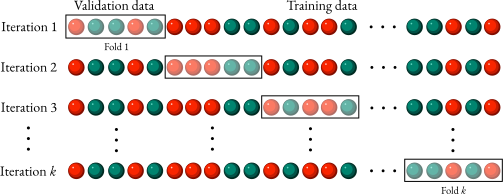
\includegraphics[width=\textwidth]{figures/kfold-cv.pdf}
  \caption{%
    An illustration of \(k\)-fold cross-validation. The data is split into \(k\) folds (subsets). In the \(k\)th iteration, the model is fit on training data consisting of \(k-1\) folds and then applied to the held-out validation data in fold \(k\), on which an error is computed. A final cross-validation error is then computed by averaging the error across all of the iterations.
    This figure is an edited version of an illustration by Gufosowa (via Wikimedia Commons, licensed under CC BY-SA 4.0).
  }
  \label{fig:k-fold-cv}
\end{figure}

For the lasso, it is typical to construct a grid of 100 \(t\) values, which means that we have to, for instance, fit \(100k\) lasso models if we use cross-validation. This can easily become computationally expensive, especially if either or both of \(n\) and \(p\) are large. In the case of the elastic net and SLOPE, the problem is complicated further since we then have \(\alpha\) or \(q\) to optimize over as well. As a result, it is vital that there are efficient methods for fitting these models, which is the topic of the following two sections. In \Cref{sec:optimization}, we discuss the various optimization methods that we can use to solve the lasso, the elastic net, and SLOPE. And in \Cref{sec:screening-rules}, we introduce the concept of \emph{screening rules}, which have been a game changer in the high-dimensional context.

\section{Optimization}\label{sec:optimization}

In the previous section we introduced the statistical models that this thesis will revolve around: the lasso, the elastic net, and SLOPE. They feature many interesting theoretical properties, which we have touched upon briefly, but it is actually not these properties that we will concern ourselves with in this thesis. Instead, we will be interested in the \emph{numerical} aspects of these problems. That is: how do we actually solve them? And, moreover, how do we do this as efficiently as possible?

As we have seen, fitting these models to data is equivalent to solving optimization problems and we have so far assumed that this is possible and that we, as a result, can recover their optima. This assumption is by no means wrong: methods for fitting the lasso, elastic net, and SLOPE are readily and freely available in many programming languages and across all major operating systems. Installing and running them amounts to only a few lines of code. To fit the full lasso path to the diabetes data that we encountered previously~(\Cref{fig:lasso-path}), for instance, we need only to call the following \lang{R}~\parencite{rcoreteam2024} code, which loads the necessary \lang{R} package \pkg{lars}, imports the dataset \data{diabetes}, and fits the lasso path to the data:

\begin{lstlisting}[language=R]
library(lars)
data(diabetes)
fit <- lars(diabetes$x, diabetes$y, type = "lasso")
\end{lstlisting}

Behind the scenes, however, the method invoked through these commands actually involve a complicated optimization algorithm into which considerable effort has been put in order to ensure that what you get in \texttt{fit} is reliable---and that you get it \emph{fast}.

Throughout the following sections, we will discuss various optimization methods that can be used to solve the lasso, the elastic net, and SLOPE. For simplicity, we will generally focus on the lasso and, in particular, the ordinary lasso (\(\ell_1\)-regularized least-squares regression). In general, however, the methods that we introduce here can be used to solve all of these problems, including the case when the objective that is regularized is part of the family of generalized linear models, which include, for instance, logistic , multinomial, and Poisson regression.

\subsection{Direct Methods}

The first optimization problem that we encountered in this text was ordinary least-squares regression, which we formally defined in \Cref{pb:ols}. Naively speaking, the solution to this problem is actually relatively straightforward. To start off, we let
\begin{equation}
  \label{eq:ols-obj}
  f(\vec{\beta}) = \frac{1}{2}\lVert \vec{y} - \mat{X}\vec{\beta}\rVert_2^2
\end{equation}
be the objective function that we want to minimize. Here and onwards we will omit the intercept term for simplicity but note that we can incorporate in any of the following methods. To minimize \Cref{eq:ols-obj}, we simply set the gradient of it to zero:
\[
  \begin{aligned}
    \nabla f(\vec{\beta})                & = \mat{X}^\intercal (\mat{X}\vec{\beta} - \vec{y}) = \zeros \implies \\
    \mat{X}^\intercal \mat{X}\vec{\beta} & = \mat{X}^\intercal \vec{y}.
  \end{aligned}
\]
This system\footnote{We have ignored the intercept \(\beta_0\) here for simplicity, but it could be incorporated easily by prepending a vector of ones to \(\mat{X}\).} is called the \emph{normal equations}. Solving the system in \(\beta\) yields the ordinary least squares estimate, which, for a one-dimensional problem is equivalent to locating the ``bottom'' of the function \(f(\beta)\) in \Cref{fig:1dconvexity-convex}. It might be tempting to want to simply invert \(\mat{X}^\intercal\mat{X}\) here and premultiply by both sides to yield an explicit solution of the form
\[
  \vec{\beta} = (\mat{X}^\intercal\mat{X})^{-1}\mat{X}^\intercal\vec{y}
\]
but this is typically a bad idea since the inverse need not be numerically stable or even exist. A better option is to use a method such as QR factorization and solve the resulting system through forward or backwards elimination, which is both more stable and efficient; all modern software use some variation on this approach.

Regardless, however, OLS regression can be solved directly and with accuracy at machine precision. This property is shared by ridge regression in which we can attain a solution simply by adding a diagonal matrix\footnote{This procedure refers to the \emph{unconstrained} form of ridge regression, which have not yet---but will soon---introduce.} to \(\mat{X}^\intercal\mat{X}\) and solving as before. The key reason for why this is the case is that OLS regression is a differentiable and quadratic problem, which means that it is \emph{convex} and hence has a global solution~(\Cref{fig:1dconvexity-convex}), unlike, for instance, the problem in \Cref{fig:1dconvexity-nonconvex}, which is non-convex (actually a third-degree polynomial) and hence has a local minimum.

\begin{figure}
  \centering
  \subcaptionbox{A convex and smooth function. The minimum ocurs when \(\nabla f(\beta) = 0\).\label{fig:1dconvexity-convex}}{\includegraphics[]{figures/1d-convexity-convex.pdf}}\hfill%
  \subcaptionbox{A non-convex but smooth function. The derivative offers no information about the global minimum (at \(-\infty\)).\label{fig:1dconvexity-nonconvex}}{\includegraphics[]{figures/1d-convexity-nonconvex.pdf}}\hfill%
  \subcaptionbox{A convex but non-smooth function. There is a global minimum, but the derivative does not exist at this point.}{\includegraphics[]{figures/1d-convexity-nonsmooth.pdf}}
  \caption{%
    Three different kinds of functions. We show the objective value \(f(\beta)\) and the gradient \(\nabla f(\beta)\) for each. In each case, our objective is to find the minimum of the function. Only the first and last are convex (the complete line segment between two points on the function lies above the function) and have a global minimum.
  }
  % \label{fig:1d-convexity}
\end{figure}

All the problems that we have covered so far: ordinary least-squares regression, the lasso, the elastic net, and SLOPE are all convex, which is the class of problems this thesis focuses on. Being convex, however, does not necessarily mean that the problem is easy to solve. The lasso, \Cref{pb:lasso}, for instance, is a convex problem, but the involvement of the inequality constraint means that a direct solution is not readily available.

Somewhat remarkably, however, it actually \emph{is} possible to solve the lasso directly, as long as we also solve the full lasso path up to the \(t\) that we want. The class of methods that makes this possible are called \emph{homotopy algorithms} since they can be used to solve the problem for all values they are parameterized by (in this case \(t\)). The first homotopy method for the lasso was introduced by \textcite{osborne2000,osborne2000a} but it is the LARS algorithm~\parencite{efron2004}, that we already saw in action at the beginning of the section, which popularized the method for the lasso.

In essence, homotopy methods for the lasso are based on the idea that the model can be solved directly if we know the support of the solution (the identity of the non-zero coefficients). Based on this idea, we start with the empty support at \(t=0\). From this point, it is possible to say which features will become active first and at what \(t\) this happens, which makes it possible to then solve the problem (directly) a this value of \(t\). The process is repeated until the entire path has been computed. We give a rough, but slightly more formalized, description of the method in \Cref{alg:homotopy}.

\begin{algorithm}
  \caption{A rough outline of the homotopy method for the lasso path. The steps in lines 3 and 4 represent the critical aspect of the algorithm, but are omitted here for brevity. They are not, however, particularly demanding computationally. Instead, the primary costs come from the linear systems that need to be solved at each step of the path.}
  \label{alg:homotopy}
  \KwIn{$\vec{\beta}^{(0)} = \zeros$, $t \gets 0$, $\mathcal{A} = \emptyset$, $i = 0$}
  \Repeat{$|\mathcal{A}| = p$}{
  $i \gets i + 1$\;
  $t \gets$ next value for which the support changes\;
  $\mathcal{A} \gets$ support at $t$\;
  $\vec{\beta}^{(i)}_{\mathcal{A}} \gets \arg\min_{\vec{\beta} \in \mathbb{R}^{|\mathcal{A}|}} f(\vec{\beta})$\;
  $\vec{\beta}^{(i)}_{\mathcal{A}^C} \gets \zeros$\;
  }
\end{algorithm}

At the time that these methods were introduced, they offered a remarkable boost in efficiency compared to the original algorithm used by \textcite{tibshirani1996}, which consisted of an iterative method based on an algorithm by \textcite{lawson1995}, which scales badly with \(p\) and is altogether inapplicable when \(p > n\).

Since the elastic net can be recast as a lasso problem, it also means that the same homotopy methods can be used also in this case. In addition, there now also exists homotopy methods for SLOPE~\parencite{nomura2020,dupuis2023}, which comes from the SLOPE path sharing the piecewise-linear property of the lasso path (although the SLOPE path is typically more complicated and features more changes in support).

Even if these homotopy methods provide a much-wanted upgrade compared to the original method in the high-dimensional setting, it is nevertheless this domain that they ultimately struggle to deal with. The root of this problem is that there are at least \(\min(n,p)\) kinks (changes in support) along the full lasso path---and in the worst case as many as \((3^p + 1)/2\) such changes~\parencite{mairal2012}. The algorithm has to solve an equivalent number of OLS regression problems, albeit at a complexity much reduced from that of solving the full problem,\footnote{LARS, for instance, incrementally update a Cholesky factorization of the Hessian matrix \(\mat{X}^\intercal\mat{X}\).} which, in the end, means that the method has found itself outperformed by iterative optimization methods~\parencite{friedman2010}, which we will introduce in the next section.

\subsection{Iterative Optimization}\label{sec:iterative-optimization}

In iterative optimization, we start with an initial guess of the solution (usually \(\vec{\beta} = \zeros\)) and then update it step-by-step until we get ``close enough'' to the optimum.\footnote{As you might expect, defining ``close enough'' is not at all a trivial matter.} This puts them apart from the direct methods we covered in the previous section, which typically involve solving a system of equations or a similar problem and yield a solution directly and at machine precision.

\subsubsection{Gradient Descent}

It is probably fair to say that \emph{gradient descent} is the quintessential iterative optimization method. The basic idea is to update the optimization variable (\(\vec{\beta}\)) by moving in the direction of the negative gradient of the objective function (\(\nabla f (\vec{\beta})\)). For a convex objective, the negative gradient points in the direction of the global minimum, which means that we eventually reach it given appropriate choices of our step sizes (how far we move in the opposite direction of the gradient).

Technically, the idea in gradient descent is to form a second-order Taylor expansion of the objective around the current iterate \(\bvec'\),
\begin{equation*}
  f(\bvec) \approx f(\bvec') + \nabla f(\bvec')^\intercal (\bvec - \bvec') + \frac{1}{2}(\bvec - \bvec')^\intercal \nabla^2 f(\bvec')(\bvec - \bvec'),
\end{equation*}
replace the Hessian matrix \(\nabla^2 f(\bvec')\) with \(\frac {1}{\tau} \mat{I}\) in this approximation, yielding
\begin{equation*}
  f'(\bvec; \bvec') = f(\bvec') + \nabla f(\bvec')^T(\bvec - \bvec') + \frac{1}{2\tau}\lVert \bvec - \bvec'\rVert_2^2,
\end{equation*}
and then, finally, solve for \(\bvec\), which gives the gradient descent update
\[
  \bvec^+ =\argmin_{\bvec \in \mathbb{R}^p} f'(\bvec; \bvec') = \bvec' - \tau \nabla f(\bvec').
\]
The method, which is simple this step repeated in each iteration, is outlined in \Cref{alg:gradient-descent}.

Observe that the \(\tau\) we used when we replaced the Hessian with a diagonal matrix is the step size in the gradient descent algorithm. This is the key parameter in the algorithm, which controls how far we move in the direction of the negative gradient.
In \Cref{fig:gradient-descent}, we show how gradient descent works for simple problems in one and two features.

\begin{algorithm}
  \caption{Gradient descent with fixed step size. An intercept can be added by either prepending a vector of ones to \(\mat{X}\) or adding a separate update step where \(\vec{\beta}\) is held fixed.}
  \label{alg:gradient-descent}
  \KwIn{$\vec{\beta} = \zeros$, $\tau >0$}{
  }

  \Repeat{convergence}{
    $\bvec \gets \bvec - \tau \nabla f(\bvec)$\;
  }
\end{algorithm}

\begin{figure}[htpb]
  \centering
  \subcaptionbox{A one-dimensional problem. The black curve shows the value of the objective \(f(\beta)\).}{\includegraphics[]{figures/gd-1d.pdf}}\hspace*{1cm}%
  \subcaptionbox{A two-dimensional problem. The grey curves are the level curves of the OLS regression objective \(f(\vec{\beta})\).}{\includegraphics[]{figures/gd-2d.pdf}}
  \caption{%
    Gradient descent in one and two dimensions. In each case the algorithm starts at \(\vec{\beta}^{(0)}\) and then proceeds towards the optimum \(\vec{\beta}^*\) (\optimum).
    The quadratic approximation of the first step is drawn in blue lines (and its optimum marked by a blue dot).
  }
  \label{fig:gradient-descent}
\end{figure}

\subsubsection{Projected Gradient Descent}

The problem for us, however, is that the lasso, the elastic net, and SLOPE---the problems we are mainly concerned with---have inequality constraints, which gradient descent cannot handle directly.
A natural alternative, however, exists in the form of \emph{projected} gradient descent. The method consist of simply taking a gradient descent step, as in \Cref{alg:gradient-descent}, and then projecting the result onto the feasible region (if the update after the gradient step is infeasible). The update is then
\[
  \bvec \gets \proj_{C}\left(\bvec - \tau \nabla f(\bvec)\right)
\]
where
\begin{equation}
  \label{eq:projection}
  \proj_{C}(\vec{u}) = \argmin_{v \in C} \lVert \vec{v} - \vec{u}\rVert_2
\end{equation}
is the projection operator that projects \(\vec{u}\) onto the feasible region \(C\). For the lasso, for instance, \(C\) is the \(\ell_1\) norm ball~(\Cref{fig:lasso-ball}), while for SLOPE it is the sorted \(\ell_1\) norm ball~(\Cref{fig:slope-balls}). The method is outlined in \Cref{alg:projected-gradient-descent} and is identical to the gradient descent algorithm (\Cref{alg:gradient-descent}), except that we have now wrapped a projection operator around the gradient descent update.

\begin{algorithm}
  \caption{Projected gradient descent. The projection operator \(\proj_C(\cdot)\) is defined in \Cref{eq:projection}.}
  \label{alg:projected-gradient-descent}
  \KwIn{$\vec{\beta} = \zeros$, $\tau > 0$}{}
  \Repeat{convergence}{
    $\bvec \gets \operatorname{proj}_{C}\left(\bvec - \tau \nabla f(\bvec)\right)$\;
  }
\end{algorithm}

\Cref{fig:projected-gradient-descent} shows the method in action for a two-dimensional lasso problem. Note how the gradient step (dotted lines) takes the algorithm outside the feasible region and that the projection step (solid lines) then moves the solution back to the feasible region.

\begin{figure}[htpb]
  \centering
  \includegraphics[]{figures/proj-gradient-2d.pdf}
  \caption{%
    Projected gradient descent for a two-dimensional lasso problem. The gray curves are the level curves of the ordinary least-squares objective \(f(\vec{\beta})\) and the blue diamond shape is the \(\ell_1\) norm constraint. The algorithm starts at \(\vec{\beta}_0\) and then proceeds towards the solution \(\vec{\beta}^*\). Each step consists of a gradient step (dashed lines) and a projection step (solid lines).
  }
  \label{fig:projected-gradient-descent}
\end{figure}

The efficiency of projected gradient descent hinges on the efficiency with which the projection can be computed. Thankfully, there exists efficient projections for both the \(\ell_1\)~\parencite{duchi2008} and sorted \(\ell_1\) norms~\parencite{zeng2015,li2021,perez2022,davis2015}, which means that the method is quite efficient for both the lasso and SLOPE.

\subsubsection{The Subgradient Method}

Projected gradient descent attacks our optimization problems by tackling the inequality constraints directly; but the by far most popular approach for solving these problems actually takes a different route by transforming the constrained problem into an unconstrained one. The idea is that we can achieve an equivalent regularization effect by, instead of constraining the solution directly, penalizing the coefficients via the objective function.

In other words, we turn the problem
\[
  \begin{aligned}
     & \text{minimize}   &  & g(\bvec),       \\
     & \text{subject to} &  & h(\bvec)\leq t,
  \end{aligned}
\]
into
\[
  \begin{aligned}
    \text{minimize} &  & f(\bvec) = g(\bvec) + h(\bvec).
  \end{aligned}
\]
In the case of SLOPE, for instance, the unconstrained version of \Cref{pb:slope} then becomes
\[
  \begin{aligned}
    \text{minimize} &  & \frac{1}{2} \lVert \vec{y} - \mat{X}\vec{\beta}\rVert + \sum_{j=1}^p \lambda_j |\beta_{(j)}|.
  \end{aligned}
\]

You may wonder what good this did us, but the key is that the we have now gotten rid of the constraint, which means that we can focus on minimizing the objective directly. We can see how the two optimization problems compare for an equivalent setting of \(\lambda\) (in the case of the unconstrained problem) and \(t\) (in the case of the constrained problem) for the lasso in \Cref{fig:constrained-unconstrained}.

\begin{figure}[tpb]
  \centering
  \subcaptionbox{The constrained form of the lasso. The level curves show the ordinary least-squares objective. The blue region is the \(\ell_1\)-norm constraint}{\includegraphics[]{figures/constrained.pdf}}\hspace*{0.8cm}%
  \subcaptionbox{The unconstrained form of the lasso. Here, the level curves show the unconstrained optimization objective.}{\includegraphics[]{figures/unconstrained.pdf}}
  \caption{%
    Constrained and unconstrained versions of the lasso. The equivalence between the problems is obtained by setting \(t = \lVert \vec{\beta}\rVert_1\) after solving the unconstrained problem to convergence for a given \(\lambda\).
  }
  \label{fig:constrained-unconstrained}
\end{figure}

The bad news is that the new objective is no longer differentiable, which means that we cannot, for example, use gradient descent with the new formulation either. The good news, however, is that there is a generalization of the derivative that can be used in the non-differentiable case, namely the \emph{subdifferential}.

The subdifferential of a function \(f\) at a point \(\vec{\beta}\) is the set of all \emph{subgradients} of \(f\) at that point. This means that the subdifferential is a set, rather than a single vector. A subgradient at a point \(\vec{\beta}\) is a vector \(\vec{g}\) such that
\[
  f(\vec{\beta}') \geq f(\vec{\beta}) + \vec{g}^\intercal (\vec{\beta}' - \vec{\beta}).
\]
In plain terms, this simply means that the linear approximation of the function at \(\vec{\beta}\) always underestimates the function. If the function is differentiable, then the subdifferential is a singleton, containing only the gradient of the function.
In \Cref{fig:lasso-subgradients}, we show some of the subgradients of a one-dimensional lasso problem.

\begin{figure}[htpb]
  \centering
  \subcaptionbox{Subgradients of a one-dimensional lasso problem. At \(\beta = 3\), there is just a single subgradient: the (ordinary) gradient, but at \(\beta =0\), there are multiple subgradients.\label{fig:lasso-subgradients}}{\includegraphics[]{figures/lasso-subgradients.pdf}}\hfill%
  \subcaptionbox{The \(\ell_1\) norm (absolute value) of the coefficient \(\beta\) and its subgradient \(\partial \lVert \beta\rVert_1\).\label{fig:l1norm-subgradient}}{\includegraphics[]{figures/l1norm-subgradients.pdf}}\hfill%
  \caption{%
    Subgradients of the lasso and the \(\ell_1\) norm
  }
\end{figure}

The existence of subgradients presents us with an intuitive solution to the problem of minimizing non-differentiable functions: use gradient descent, but replace the gradient with the subgradient, and take a step in its direction. We outline the algorithm in \Cref{alg:subgradient-method}.

\begin{algorithm}
  \caption{The subgradient method. Note that \(g\) can be \emph{any} subgradient of the subdifferential \(\partial f(\beta)\).}
  \label{alg:subgradient-method}
  \KwIn{$\vec{\beta} = \zeros$, $\tau > 0$}{
  }
  \Repeat{convergence}{
    $\vec{s} \gets \vec{s} \in \partial f(\bvec)$\;
    $\bvec \gets \bvec - \tau s$\;
  }
\end{algorithm}

The attractiveness of the subgradient method is that it is general and works for a large class of problems, including the lasso, the elastic net, and SLOPE. The problem is that it converges slowly and is therefore never used in practice for these problems.

\subsubsection{Proximal Gradient Descent}

Fortunately, we have structure in this problem that we have yet to exploit, namely that although \(f = g + h\) is not differentiable, \(g\) in fact \emph{is}. Based on this, one idea is to simply leave \(h\) alone and minimize the quadratic expansion of \(g\) plus \(h\) (untouched).
\begin{multline*}
  \argmin_{\bvec} \left( g(\bvec') + \nabla g(\bvec')^\intercal(\bvec - \bvec') + \frac{1}{2\tau}\lVert \bvec - \bvec'\rVert_2^2 + h(\bvec) \right) \\
  = \argmin_{\bvec} \bigg( \frac{1}{2\tau}\lVert \bvec - \big(\underbrace{\bvec' - \tau \nabla g(\bvec')}_{\text{Gradient update}}\big)\rVert_2^2 + h(\bvec)\bigg).
\end{multline*}

Let us call the function that solves this problem the \emph{proximal operator} of \(h\), denoted \(\prox_{h,\tau}\), and define it as
\[
  \prox_{h,\tau}(\vec{u}) = \argmin_{\vec{v}} \left( \frac{1}{2\tau}\lVert \vec{v} - \vec{u}\rVert_2^2 + h(\vec{v}) \right).
\]
The proximal operator is a generalization of the projection operator that we introduced earlier, and we can obtain the latter by using the indicator function of the feasible region as the function \(h\). We outline the basic version of the proximal gradient descent algorithm in \Cref{alg:pgd}.

\begin{algorithm}[hbtp]
  \caption{Proximal gradient descent. Note that the gradient is taken with respect to \(g\) and not \(f\) (for which it does not exist).}
  \label{alg:pgd}
  \KwIn{$\vec{\beta} = \zeros$, $\tau > 0$}{}
  \Repeat{convergence}{
    $\bvec \gets \prox_{h, \tau}\left(\bvec - \tau \nabla g(\bvec)\right)$\;
  }
\end{algorithm}

The reason for why all of this works is that the proximal operator has an explicit, and often efficient, form for all the problems we are interested in solving here. For the lasso, for instance, the proximal operator has a particularly simple form:
\[
  \prox_{h,\tau}(\vec{u})  = \argmin_{\vec{v}} \left( \frac{1}{2\tau}\lVert \vec{v} - \vec{u}\rVert_2^2 + \lambda \lVert \vec{v} \rVert_1 \right)
  = \st_{t\lambda}(\vec{u}),
\]
where
\[
  \st_{\lambda}(\vec{u})_i = \sign(u_i)\max(\lvert u_i \rvert - \lambda, 0),
\]
is the \emph{soft-thresholding operator}~\parencite{donoho1995} and is illustrated in \Cref{fig:soft-thresholding}. Using proximal gradient descent for the lasso is also known as the iterative shrinkage-thresholding algorithm (ISTA)~\parencite{beck2009}.

\begin{figure}[htpb]
  \centering
  \includegraphics[]{figures/soft-thresholding.pdf}
  \caption{%
    The soft-thresholding operator: the proximal operator in the case of the lasso. Here we show it for three different values of \(\lambda\). For \(\lambda = 0\), there is no thresholding (penalization), and the operator becomes the identity function. For all other values, the operator shrinks its input toward zero. For \(|u| \leq \lambda\), the output is exactly zero.
  }
  \label{fig:soft-thresholding}
\end{figure}

Proximal gradient descent has a long history. \textcite{rockafellar1970} was responsible for much of the early work. \textcite{nesterov1983} introduced the first accelerated version of proximal gradient descent algorithms, which where later improved upon by, for instance, \textcite{beck2009} in the form om the fast iterative shrinking-thresholding algorithm (FISTA). Other improvements include stochastic versions, line searches, improved step size settings, and other types of accleration, such as the Anderson variant~\parencite{mai2020}.

At this point you may wonder what we have gained compared to the projected gradient method. For one thing, we have obtained an algorithm with more general applicability. Indeed, as \textcite{bogdan2015} showed, there is an efficient algorithm for computing the proximal operator even in the case of the sorted \(\ell_1\) norm. Furthermore, we have also gained slightly in computational efficiency. In the lasso case, for instance, the soft-thresholding operator has \(\mathcal{O}(p)\) complexity whereas the projection onto the \(\ell_1\) ball has \(\mathcal{O}(p\log p)\) complexity. Please see \Cref{fig:lasso-projgrad-comp} for a small example on what this can amount to in practice.

\begin{figure}[htpb]
  \centering
  \includegraphics[]{figures/lasso-projgrad-comp.pdf}
  \caption{%
    Comparison between projected and proximal gradient descent for an equivalent lasso problem.
    Per-iteration, the methods both perform almost on par with one another. In terms of wall-clock time, however, the proximal method is more efficient.
  }
  \label{fig:lasso-projgrad-comp}
\end{figure}

In conclusion, proximal gradient descent is a simple algorithm with strong convergence guarantees that is easy to implement. As we shall see next, however, it is typically outperformed by a more naive method: coordinate descent.

\subsubsection{Proximal Coordinate Descent}

Coordinate descent is a simple algorithm: update one coefficient (coordinate) at a time by finding the minimizer with respect to that coefficient. In other words, we solve a one-dimensional problem at each iteration of the algorithm. The algorithm extends naturally to the case when we have a composite objective of the form \(f = h + g\), as in the case of proximal gradient descent, provided that \(h\) is differentiable and \(g\) is convex and \emph{separable} in \(\bvec\). Formally, this algorithm is called \emph{proximal coordinate descent}. In this text, however, we will also allow ourselves a slight misuse of nomenclature and simply call it \emph{coordinate descent}. The basic outline of the algorithm is given in \Cref{alg:pcd}.

\begin{algorithm}[hbtp]
  \caption{Proximal coordinate descent. Note that the implementation given here is designed for illustration; many improvements can be made that are critical to the practical performance of the algorithm.}
  \label{alg:pcd}
  \KwIn{$\vec{\beta} = \zeros$, \(\vec{\tau} \in \mathbb{R}^p_+\)}
  \Repeat{convergence}{
    Pick \(j \in \{1, 2, \dots, p\}\)\;
    $\beta_j \gets \prox_{h,\tau}\left(\beta_j - \tau_j \nabla g(\bvec)_j\right)$\;\label{alg:pcd-update}
  }
\end{algorithm}

For the lasso, the coordinate descent update in \Cref{alg:pcd-update}~(\Cref{alg:pcd}) is particularly cheap and amounts only to soft-thresholding of the partial residual. In \Cref{fig:pcd-lasso}, we show a simple example of how coordinate descent works for a two-dimensional lasso problem.

\begin{figure}[htpb]
  \centering
  \includegraphics[]{figures/cd.pdf}
  \caption{%
    Cyclic coordinate descent for a lasso problem in two dimensions. At each step, we minimize only in the direction of one of he coefficients (along either the x or the y axis). In this case, \(g\) is the least-squares criterion, which means that the step always takes us to the minimum in that direction.
  }
  \label{fig:pcd-lasso}
\end{figure}

There are varies strategies for picking the coefficient to optimize over in step three. The simplest and most common alternative is to cycle through the coefficients one by one, which is called \emph{cyclic} coordinate descent. Another common alternative is to pick the coefficient at random, which makes for an algorithm that is easier to analyze than cyclic coordinate descent and somewhat more robust, but which also, in our experience, usually slightly slower.

At face-value it may seem somewhat surprising that this simple strategy should outperform proximal gradient descent, which considers all features simultaneously, particularly in light of the fact that proximal gradient descent sports better convergence rates~\parencite{wright2015}. Yet, barring a few exceptions, this is precisely the case~(\Cref{fig:cd-vs-pgd}).

\begin{figure}[htpb]
  \centering
  \includegraphics[]{figures/cd-vs-pgd.pdf}
  \caption{%
    Proximal coordinate descent versus accelerated proximal gradient descent~(FISTA) for two datasets: \data{news20}~\parencite{keerthi2005} and \data{RCV1}~\parencite{lewis2004}. The dimensions of the data are $n=\num{199961}$, $p=\num{355191}$ for \data{news20} and $n = \num{20242}$,  $p=\num{47236}$ for \data{RCV1}. The response in both cases is binary and we fit a standard lasso model In both cases we normalize with maximum--absolute value scaling. The comparisons were made using the \pkg{benchopt} package~\parencite{moreau2022a}.
  }
  \label{fig:cd-vs-pgd}
\end{figure}

The counterintuitive nature of this result may explain why coordinate descent algorithms were initially largely ignored in the literature on optimization. \textcite{shevade2003,fu1998a, daubechies2004} all wrote (relatively) early papers on coordinate-descent algorithms for the lasso, yet these initially received scant attention. It was only several years later that a paper by \textcite{friedman2007} and corresponding software implementation in the \lang{R} package \pkg{glmnet}~\parencite{friedman2010} caused the method to grow in popularity.

The main reason for why coordinate descent works so well for the lasso, the elastic net, and many related problems is related to the size of the steps that the algorithms can take (while still guaranteeing convergence). In the least-squares case, proximal gradient descent is limited by a step size of \(\tau = 1/\lVert \mat{X}\rVert_2\), whereas coordinate descent can take steps of size \(\tau_j =1/\lVert \vec{x}_j \rVert_2^2\), which for much real data are decidedly larger for many of the features and hence promote faster convergence. For \data{news20}, for instance, we have \(\lVert \mat{X}\rVert_2 = 161\) whereas the median of \(\{\lVert \vec{x}_j\rVert_2^2 : j = 1,2,\dots,p\}\) is \(1.40\) (interquartile range: 1.26--1.60, maximum: 34.4). The price we pay for this increase in step size is a limit to one direction at a time. This can pose problems in the case when there is large correlation between some features, since coordinate descent then may struggle to break this dependency apart.\footnote{Note that proximal gradient descent is also not well-equipped to deal with this situation. Instead, this is the setting where Hessian-based methods such as proximal Newton~\parencite{lee2014} dominate.} Empirically, however, we have found coordinate descent to largely dominate proximal gradient descent.

As in the case proximal gradient descent, coordinate descent can also be accelerated via the Nesterov scheme~\parencite{nesterov1983} or Anderson acceleration~\parencite{bertrand2021}. In practice, however, we have found that the benefit of acceleration is lower in the case of coordinate descent than it is for gradient descent.

% Another way to look at it is to recognize that, in the standard lasso case (when \(g\) is the OLS objective) coordinate descent actually solves the one-dimensional problem \emph{exactly} at each step, which is not the case for proximal gradient descent. In other words: coordinate descent uses more information about the problem, including the curvature of the optimization surface (in the direction of the current coordinate).

One problem with coordinate descent, however, is that it requires the objective to be separable in the optimization variable \(\vec{\beta}\); this is not the case for SLOPE, which makes the method inapplicable for this problem.

%In paper~\V~\parencite{larsson2023}, however, we present a way to tackle this problem by using a hybrid of coordinate descent and proximal gradient descent.

We have introduced many optimization methods in this section, yet have only scratched the surface in the field. Several methods have been omitted, such as the alternating direction method of multipliers (ADMM)~\parencite{boyd2010}, proximal Newton~\parencite{lee2014}, interior-point methods~\parencite{kim2007}, and stochastic gradient descent~\parencite{robbins1951,bottou2010} and its many derivatives. We have also omitted many details regarding the implementation of the algorithms, such as step size selection and convergence criteria. Yet, while these are important and interesting aspects of the algorithms, we omit them here for brevity and provide all the necessary details in the papers themselves.

Although optimization algorithms are fundamental in ensuring good performance in fitting sparse regression models such as the lasso, the elastic net, and SLOPE, they are not the only way to improve performance. In the next section, we will introduce \emph{screening rules}, which drastically reduces the computational cost of fitting these models, particularly in the high-dimensional setting.

\section{Screening Rules}\label{sec:screening-rules}

Screening rules are a remarkably efficient method for speeding up the optimization of sparse regression methods. They are based on the following reasoning:
\begin{enumerate}
  \item We know that the solution is going to be sparse, especially if \(p \gg n\)\footnote{Recall, for instance, that the lasso can only select \(\min(n, p)\) features.}.
  \item We also know something about the importance of the features, even before fitting the model, since we for instance (as in \Cref{fig:sparse-signal}) can compute the correlation between the features and the response. In addition to this, we are also typically interested in solving for a range of regularization parameters, which means that the problem we are currently trying to solve is likely related to a problem we have already solved.
  \item Therefore, we might be better of by only considering a subset of the features when solving the problem. And if this subset is small and selecting it is cheap, then we should be able to save a lot of time.
\end{enumerate}
This intuition turns out to be correct, and screening rules have consequently brought a pivotal discovery to the field of optimization for sparse methods, particularly in the high-dimensional domain.

The first screening rule for the lasso, SAFE~(SAfe Feature Elimination), was introduced by \textcite{elghaoui2010}. In essence, the authors showed that it was possible to confine the solution for a given \(\lambda\) to a region of the feature space, and feature-by-feature ascertain whether it is possible for the feature be selected in the solution.

In practice, this means that if you have a dataset of, say, one million features (\(p\)) and one thousand observations (\(n\)) and want to fit the lasso for some value of \(\lambda\), then there is a good chance that you may just have to fit a problem with a few hundred features, while at the same time guaranteeing that you will reach the same solution as the one-million-feature problem would. In addition, the cost of running the screening rule is negligible next to solving the problem (even the reduced problem). The net result is a remarkable gain in computational performance. It is not in our experience rare to see speedups of several orders of magnitude, for instance reducing the time taking to fit this size of model from hours to minutes (or even less).

The screening rule introduced by \textcite{elghaoui2010} is a \emph{safe} screening rule, meaning that all of the features discarded by the rule are guaranteed to be absent at the optimum. As it turns out, however, this requirement on safety in general leads to rules that are overly conservative. This was made clear in a paper by \textcite{tibshirani2012}, in which they introduced the \emph{strong screening rule for the lasso}. This rule uses an initial screening test that is \emph{heuristic} (as opposed to safe), which means that it may discard features that actually are part of the solution. This necessitates a check of the optimality conditions after solving the reduced problem and, in case any features were incorrectly discarded, a refitting of the model with these features icluded. As the authors showed, however, these \emph{violations} of the screening rule are so rare in practice that there is often no need to refit. And if there is, the estimate from the reduced problem is often so close to the optimum of the real problem that only a few extra iterations of the optimization algorithm are needed.

It is important to highlight that the nomenclature for screening rules is quite misleading.\footnote{We stress this point since we have (repeatedly) found this fact to stump reviewers of our papers.} Even if the screening performed by the strong rule is \emph{not} safe, the actual screening rule method \emph{is}, which stems directly from the fact that all of these methods include checks of the optimality conditions in order to safeguard against discarding features that are part of the solution.\footnote{There \emph{are} screening rules that actually are unsafe, but they are used for an altogether different purpose in which one is interested not just in screening, but also changing the model (for instance the lasso) itself.} In other words, even though we call some rules \emph{safe} and some \emph{heuristic}, they are in fact \emph{all} safe as they are implemented in practice.

\textcite{tibshirani2012} also introduced the notion of \emph{sequential} screening rules, meaning that screening is performed along the regularization (lasso) path with the solution at the current step on the path as the starting point for the screening rule, which significantly impoves the effectiveness of the rule. One problem with both SAFE and the strong rule, however, is that their effectiveness decrease when features in the design are heavily correlated---the problem is particularly severe in SAFE. This lead \textcite{tibshirani2012} to conclude, which they also demonstrate empirically, that the most efficient screening method (at least in the sequential case) is to begin with the set of features that have so far \emph{ever} been active along the path: \(\mathcal{E}\), and solve the problem for this set first. After reaching a solution for this set, the optimality checks are then performed on the features present in the strong rule set \(\mathcal{S}\), but not in \(\mathcal{E}\) (\(\mathcal{S} \setminus \mathcal{E}\)). If there are any violations, which is often the case since no screening was performed, these features are entered into \(\mathcal{E}\). The problem is then solved, again, but this time for the updated \(\mathcal{E}\). This procedure is then repeated until no violations are found among \(\mathcal{S} \setminus \mathcal{E}\). Finally, when this happens, the optimality conditions are checked for the entire set of features, and if no violations are found, the solution is deemed to be found. If there are violations, the procedure repeats with these features added to \(\mathcal{E}\).

Since these two papers were published, there has been a slew of research around screening rules for the lasso as well as other sparse regression problems. Other notable examples of safe rules include the sphere tests~\parencite{xiang2011},
R-region test~\parencite{xiang2012}, and
Gap~Safe~\parencite{fercoq2015,ndiaye2017}.

We have so far discussed screening rules in relatively informal terms. In the next section, we will provide a more formal treatment of the topic, which we hope will provide a better understanding of how the methods work.

\subsection{Screening Rules and the Correlation Vector}

To better understand how screening rules work, we need to consider the optimality conditions of our problems. For the unconstrained versions of our problems, they are
\begin{equation*}
  % \label{eq:stationarity}
  \boldsymbol{0} \in \nabla g(\bvec) + \vec{s} h(\bvec),
\end{equation*}
where \(\vec{s}\) is a subgradient of the penalty term \(h\). Letting \(\vec{c} = -\nabla g(\bvec)\), we can rewrite this as
\begin{equation}
  \label{eq:kkt-check}
  \vec{c} \in \vec{s} h(\bvec).
\end{equation}
We will call \(\vec{c}\) the \emph{correlation vector}, which is simply the negative gradient of \(g(\bvec)\) with respect to \(\vec{\beta}\).

For illustrative purposes, we will focus on the lasso here, for which the \(\partial h(\bvec)\) is the subdifferential of the \(\ell_1\) norm multiplied with \(\lambda\), defined as
\[
  s_j \in
  \begin{cases}
    \{
    \lambda\sign(\hat\beta_j)\} & \text{if } \hat\beta_j \neq 0, \\
    [-\lambda, \lambda]         & \text{otherwise},
  \end{cases}
\]
which we previously visualized in \Cref{fig:l1norm-subgradient}.
One consequence of this is that, if
\begin{equation*}
  |\nabla g(\vec{\beta})_j| < \lambda,
\end{equation*}
then it must also hold that \smash{\(\beta_j^* = 0\)}. In other words, if the absolute value of the gradient with respect to feature \(j\) is smaller than our level of regularization, then the feature must be absent from the solution. Similarly, this also means that if \smash{\(\beta_j^* \neq 0\)}, then its gradient will be \(\pm \lambda\). We can observe this behavior in \Cref{fig:cor-coef-lasso-path}, where we have plotted the lasso path for the diabetes dataset that we have encountered before. Note that we start at the left. At this point only a single feature is active. Then, as we lower \(\lambda\) (move from left-to-right in the plot), the features become active one-by-one. And at exactly the point where they do so, they also join either of the lines \(c = \pm \lambda\); and as long as they stay active, that is where they remain.

\begin{figure}[htpb]
  \centering
  \includegraphics[]{figures/cor-coef-lasso-path.pdf}
  \caption{%
    The lasso path for the diabetes data. This time, we have also plotted the correlation (negative gradients) along the path. In order for a feature to become active from one step on the path (one value of \(\lambda\)) to the next, its correlation \(c_j\) has to reach either of the \(\lambda = \pm c\) (dotted) lines. Note that the x-axis is flipped to illustrate the fact that we typically proceed from a large \(\lambda\) towards a small one (left to right in the plot).
  }
  \label{fig:cor-coef-lasso-path}
\end{figure}

So, if we knew, before fitting, that \(|c_j| < \lambda\), then we could safely discard feature \(j\) from the problem and still solve it as if it were always there. The problem, however, is that we do not have access to the correlation vector before fitting the model.

What we can do instead, however, is to estimate the correlation vector and use that in the place of the true value. Let us say that we are at step \(k\) on the path and have computed the solution at this step; then we also know \(\vec{c}\) at this step (\(\vec{c}^{(k)}\)). Next, we want to predict what \(\vec{c}^{(k+1)}\) will be in order to screen features for this (upcoming) step. One rather conservative approach for this is to assume that gradient of the correlation vector is bounded by one, in other words, we introduce the approximation
\[
  \hat{c}_j^{(k+1)} = c_j^{(k)} + \sign\left(c_j^{(k)}\right)\left(\lambda_k - \lambda_{k+1}\right).
\]
Using this approximation is in fact exactly the strong rule for the lasso. In \Cref{fig:strong-rule}, we illustrate what this approximation amounts to in practice for the diabetes dataset.

\begin{figure}[htpb]
  \centering
  \includegraphics[]{figures/strong-rule.pdf}
  \caption{%
    The sequential strong rule for the lasso. The data is the diabetes dataset that we have encountered several times already. We are at step \(k\) and want to screen features for step \(k+1\). We show the screening rule for two features here. The filled circles show \(|c_j|\) for each feature and the open circles show the strong rule estimate \(|\hat{c}_j|\). For feature 1, the approximation \(|\hat{c}_1|\) does not reach \(\lambda\) in time for the next step---so the rule discards it. For the fourth feature, however, \(|\hat{c}_4|\) is larger than \(\lambda\), and so feature 4 cannot be discarded.
  }
  \label{fig:strong-rule}
\end{figure}

As we mentioned previously, this is a somewhat conservative estimate of the gradient for the next step, which, in addition, uses no information at all about the shape of the path of the correlation vector. And even though the rule has lead to remarkable improvements in performance of optimization algorithms, this fact causes it to struggle in less well-conditioned datasets where, for instance, there is large correlation between the features~\parencite{tibshirani2012}.

Another consequence of \Cref{eq:kkt-check} is that it is possible to know at which \(\lambda\) the first feature enters the model. In the case when \(g\) is the least-squares objective, for instance, we have the following optimality condition:\footnote{Note that this equation is for the no-intercept case.}
\[
  \left|\mat{X}^\intercal\left(\vec{y} - \mat{X}\vec{\beta}\right)\right| = |\mat{X}^\intercal \vec{y}| \leq \lambda
\]
since we know that \(\bvec = \zeros\) at this point. This means that the largest value for this equation to hold is
\[
  \lambda_\text{max} = \max_j |\vec{x}_j^\intercal \vec{y}|.
\]
We have used this setting repeatedly throughout this text as a starting point for the lasso path (in the unconstrained case).

This also, however, highlights a property of the lasso that is true of the elastic net and SLOPE as well: it is sensitive to the scales of the features. The larger the values of \(\vec{x}_j\), the larger the inner product \smash{\(\vec{x}_j^\intercal \vec{y}\)} becomes, which means that if feature \(j\) for instance is the length of a person, then it will enter the path earlier if our measurements are in meters rather than centimeters. This is of course not desireable. To deal with this issue, we need to \emph{normalize} the features, which is the topic of the next section.

\section{Normalization}\label{sec:normalization}

One important aspect of regularized models is that they are generally sensitive to the scale of the features in the problem. This is the case for the lasso, the elastic net, and SLOPE, since they penalize the magnitude of the coefficients. And it puts them apart from ordinary least squares and best-subset selection, which we introduced earlier.

For a simple example of this behavior, assume that we have a dataset that is generated from a normal distribution in the following manner:
\[
  \mat{X} \sim \operatorname{Normal}\left(\begin{bmatrix}0 \\ 0\end{bmatrix}, \begin{bmatrix} 4 & 0 \\ 0 & 1\end{bmatrix}\right), \qquad \vec{\beta} = \begin{bmatrix} 1/2 \\ 1 \end{bmatrix}, \qquad \vec{y} = \mat{X}\vec{\beta} + \vec{\varepsilon},
\]
with \(\varepsilon \sim \normal(0,1)\), identically and independently for each \(i = 1,2,\dots,n\).

In other words, we have generated our features from two normally distributed variables, both with mean zero and standard deviation 2 and 4, respectively, and with no correlation between them. We have constructed our problem such that the effects on the response for the two features are equivalent, in the sense that a change of one standard deviation in either feature will result in a change of one in the response.

Since the errors are generated according to the assumptions of the ordinary least squares model, we will recover the true coefficients in expectance. And when we compute the standardized coefficients from our estimates, according to
\[
  \hat{\beta}_\text{std} = s_j\hat{\beta}_j,
\]
where \(s_j\) is the standard deviation of the feature \(\vec{x}_j\), the coefficients are both 1 (for ordinary least-squares regression).

If we fit the lasso to this data, however, we will find that the feature with the larger standard deviation will be penalized \emph{less} than the other~(\Cref{tab:normalization-coefficients}), which we see from looking at the standardized coefficients. A similar effect occurs in ridge regression. This behavior is typically not desirable.

\begin{table}[hbtp]
  \caption{The effect of regularization on the regression coefficients and standardized versions thereof. }
  \label{tab:normalization-coefficients}
  \centering
  \begin{tabular}{lcc}
    \toprule
    Model & \(\hat{\vec{\beta}}\)                                  & \(\hat{\vec{\beta}}_\text{std}\)                      \\
    \midrule
    OLS   & \(\begin{bmatrix} 0.50 & 1.00\end{bmatrix}^\intercal\) & \(\begin{bmatrix}1.00 & 1.00\end{bmatrix}^\intercal\) \\ \addlinespace
    Lasso & \(\begin{bmatrix} 0.38 & 0.50\end{bmatrix}^\intercal\) & \(\begin{bmatrix}0.75 & 0.50\end{bmatrix}^\intercal\) \\ \addlinespace
    Ridge & \(\begin{bmatrix} 0.47 & 0.78\end{bmatrix}^\intercal\) & \(\begin{bmatrix}0.93 & 0.78\end{bmatrix}^\intercal\) \\ \addlinespace
    \bottomrule
  \end{tabular}
\end{table}

To tackle this, the standard approach is to \emph{normalize} the design matrix \(\mat{X}\) before fitting the model by centering (subtracting a value, for instance its mean) and scaling each feature (by dividing with a value, for instance its standard deviation).\footnote{Afterwards, the coefficients are typically returned to their original scale.} The goal is to place the features on the same scale. For features that are normally distributed, this is relatively straightforward to do. You simply need to scale with the standard deviation. But when the distribution of the features is different, for instance when whey are binary \(x_{ij} \in \{0,1\}\), the situation is more complicated.
Unfortunately, there is little literature to fall back on in this case; in fact, this holds in general for the case of normalization. Typically, researchers and practioners instead rely on ``standard practice'', but this differs from field to field. Two common types of normalization is \emph{standardization}, which is shifting by the mean and scaling by the standard deviation\footnote{The formula without Bessel's correction is typically used.} of each feature, and \emph{max--abs} scaling, which does no shifting but scales with the maximum absolute value of each feature. The first type, standardization, is common in the statistical literature, whilst the second type, max--abs normalization, is common in machine learning, particularly when dealing with sparse data. As we can observe in \Cref{fig:normalized-realdata-lasso-paths}, however, the two methods generate starkly different results for the estimated coefficients in many datasets.

\begin{figure}[htpb]
  \centering
  \includegraphics[]{figures/realdata_paths.pdf}
  \caption{%
    Lasso paths for real datasets using two types of normalization: standardization and maximum absolute value scaling (max--abs). We have fit the lasso path to three different datasets: \data{leukemia}~\parencite{golub1999}, \data{triazines}~\parencite{king}, and \data{w1a}~\parencite{platt1998}. For each dataset, we have colored the coefficients if they were among the first five features to become active in under either of the two types of normalization schemes. We see that the paths differ with regards to the size as well as the signs of the coefficients, and that, in addition, the coefficients to become active first differ between the normalization types.
  }
  \label{fig:normalized-realdata-lasso-paths}
\end{figure}

This concludes our introduction to the topics of this thesis, including some of the issues and challenges faced by methods and practices in this field. In the next section, we will introduce the papers that this thesis is based on and briefly summarize their contributions in tackling these challenges.

\section{Summary of the Papers}

\subsection{Paper \I}

In \Cref{sec:screening-rules}, we demonstrated the considerable effect that screening rules have had on sparse regression problems in the large-\(p\) setting. As a result, the papers by \textcite{elghaoui2010} and \textcite{tibshirani2012} led to a surge in interest for screening rules for the lasso and its derivatives, including the elastic net. For SLOPE, however, there existed no screening rule until our work in this paper, in which we introduced the \emph{strong screening rule for SLOPE}~\parencite{larsson2020b}.

A key contribution in our paper is the development of a practical characterization of the subdifferential for the sorted \(\ell_1\) norm, from which we derive an effective algorithm for implementing the screening rule in practice. Just as for the lasso, we demonstrate remarkable boosts in performance for fitting SLOPE~(\Cref{tab:strong-screening-slope}). The net result is a considerable extension in reach for SLOPE in the high-dimensional setting.

\begin{table}[hbtp]
  \caption{Benchmarks measuring wall-clock time for four datasets fit with different models using either the strong screening rule or no rule.}
  \label{tab:strong-screening-slope}
  \centering
  \small
  \begin{tabular}[t]{%
      l
      l
      S[table-format=4.0]
      S[table-format=6.0]
      S[table-format=5.0]
      S[table-format=4.0]
    }
    \toprule
    \multicolumn{1}{c}{} & \multicolumn{1}{c}{} & \multicolumn{1}{c}{} & \multicolumn{1}{c}{} & \multicolumn{2}{c}{{Time (s)}}               \\
    \cmidrule(l{3pt}r{3pt}){5-6}
    Dataset              & Model                & $n$                  & $p$                  & {No screening}                 & {Screening} \\
    \midrule
    dorothea             & Logistic             & 800                  & 88119                & 914                            & 14          \\
    e2006-tfidf          & Least squares        & 3308                 & 150358               & 43353                          & 4944        \\
    news20               & Multinomial          & 1000                 & 62061                & 5485                           & 517         \\
    physician            & Poisson              & 4406                 & 25                   & 34                             & 34          \\
    \bottomrule
  \end{tabular}
\end{table}

\subsection{Paper \II}

As we saw in \Cref{sec:screening-rules}, screening rules are particularly effective when they are sequential, that is, operate along the lasso, elastic net, or SLOPE paths. But another possibility that had previously not been explored is the idea of screening not only for the next step on the path, but for \emph{all} of the remaining steps as well. This is the idea behind \emph{look-ahead screening rules}, which we introduce in this short paper~\parencite{larsson2021}. We employ this idea for the gap-safe screening rule, which, as the name suggests, is a safe screening rule. This means that if a feature is screened out, it is guaranteed to be zero in the solution.
% TODO: add a reference to gap safe rule

In \Cref{fig:paper2-highlight}, we illustrate the effectiveness of look-ahead screening for the lasso path at the first step for the \data{leukemia} dataset. What the plot indicates is that many features can be safely exempt from model fitting for a range of steps on the path, which means that we only need to re-screen them at the first grey square for each given feature.

\begin{figure}[htpb]
  \centering
  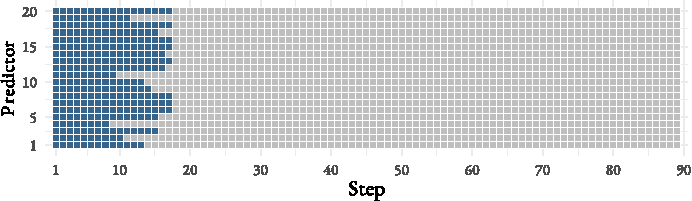
\includegraphics[]{figures/paper2-highlight.pdf}
  \caption{%
    Look-ahead screening for the lasso at the first step on the path for the \data{leukemia} dataset. The plot shows a random sample of 20 features. Blue squares indicate that the corresponding feature can be discarded for those steps on the lasso path.
  }
  \label{fig:paper2-highlight}
\end{figure}

In the paper, we show that this effect has sizeable consequences for the computation time requires for fitting the full path.

\subsection{Paper \III}

Even though the strong rule for the lasso is highly effective in general, there is one area in which it struggles, namely, when features are highly correlated. \textcite{tibshirani2012} in fact noted this themselves and forwarded it as the main motivation for using the working-set strategy (where the model is initially fit using the ever-active set, rather than the strong set).

The reason for this is that the strong rule, and every other screening rules we know of, ignores information about the gradient of the correlation vector \(\vec{c}\), even though it contains useful information about the structure of the path. Looking at \Cref{fig:strong-rule}, for instance, we see that the strong rule bound is indifferent to the slopes of the correlation vectors. This is the motivation for the \emph{Hessian screening rule} that we introduce in the third paper of the thesis~\parencite{larsson2022b}. The name stems from the fact that we use second-order information about the optimization problem, which involves the Hessian matrix \(\mat{X}^\intercal\mat{X}\). The rule offers a better estimate of the correlation vector~(\Cref{fig:paper3-highlight}), which in practice leads to better screening performance.

\begin{figure}[tpb]
  \centering
  \pgfplotsset{width=11.5cm,height=9cm}
  \input{figures/unit-slope.tikz}
  \caption{%
    An illustration of the strong and Hessian screening rules for a lasso problem. We are at \(\lambda_k\) and are looking to screen features for \(\lambda_{k+1}\). The black solid line shows the path of the correlation vector for the \(j\)th feature, which is inactive (its coefficient is zero) until the point where it joins the dashed line. In blue and orange colors, we show the predicted values for \(c_j\) between \(\lambda_k\) and \(\lambda_{k+1}\). For the strong rule, the predicted value lies above the dashed line, so it is not discarded by the rule (even though it is inactive). For the Hessian rule, however, the prediction \(\hat{c}_j\) \emph{does} lie below the dashed line, and so the feature \emph{is} discarded.
  }
  \label{fig:paper3-highlight}
\end{figure}

The screening method manages to be effective, particularly when \(g\) is the least-squares objective, because of efficient updates of the Hessian matrix and its inverse. And as a bonus, the availability of these quantities also allow for adaptively tailoring the \(\lambda\) sequence in order to better approximate the true lasso path.

\subsection{Paper \IV}

The few optimization methods that we have introduced so far amount to no more than a drop in the ocean of the vast volume of research that is the field of optimization. And although we have provided a few select benchmarks of our methods, we are still far removed from any kind of comprehensive study of their comparative effectiveness. This is not just an issue of our limited overview in this thesis, but in fact a general problem for research in optimization.

The problem is that there are now so many optimization methods to examine and so many different models and datasets on which to compare them on, that it has become difficult to keep track of which methods it is that actually do best on a given problem. You can easily find a paper A that studies optimization methods X and Y on datasets I and II and conclude that X is better than Y but then find another paper, B, which studies methods X, Y, and Z on datasets I and III and conclude that, actually, Y is better than X and by the way, Z happens to be best of them all. Then, later, you find paper C, which claims that Z actually is considerably worse than X and in fact also performs better for dataset IV. In addition to this confused state of affairs, it is commonly also the case that the authors of these papers 1) used different criteria for convergence, 2) programmed their methods in contrasting programming languages, and 3) benchmarked their experiments on different hardware.

In short, there is a dire need for a framework through which this process can be made simple, reproducible, and transparent. This is the motivation behind the \pkg{benchopt} package, which we present in the fifth of this thesis' papers~\parencite{moreau2022a}.

The goal of \pkg{benchopt} is to make life easier for both researchers in optimization and users of optimization software. For a researcher who has developed new optimization method for SLOPE, for instance, all you need to do is to write the optimization method for your algorithm and plug it into the existing \pkg{benchopt} benchmark for SLOPE and run it. The package will then automatically compare your method to all the other methods in the benchmark and output table and plots of the results~(\Cref{fig:paper4-highlight}). And if you instead are a user who is interested in using SLOPE for your applied work and want to know which algorithm to use, you can either browse the extensive database of results that other users have already uploaded or just download the benchmark and run it yourself on the data that you are interested in using it for.

\begin{figure}[htpb]
  \centering
  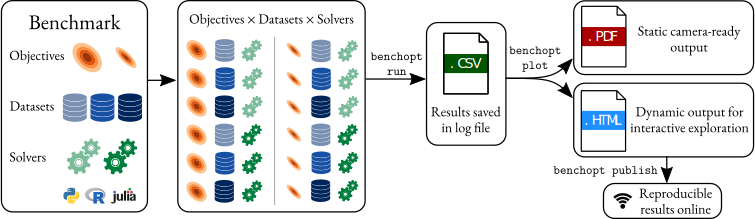
\includegraphics[width=\textwidth]{figures/benchopt_schema_objectives_with_logos.pdf}
  \caption{%
    A schematic over how a benchmark is set up and run using \pkg{benchopt}. The benchmark consists of a set of files that define an objective, datasets, and solvers. When the user runs \texttt{benchopt run}, the package combines all of the possible combinations of objectives, datasets, and solvers and outputs a neatly formatted database of the results.
    Using \texttt{benchopt plot}, the user can then easily compare the different methods through interative visualizations or produce publication-ready plots to insert directly into a paper.
    Finally, to make the results available to the \pkg{benchopt} community, the user can run \texttt{benchopt publish}, which opens up a pull-request against the public repository of benchmark results.
  }
  \label{fig:paper4-highlight}
\end{figure}

\subsection{Paper \V}

As we saw in \Cref{fig:cd-vs-pgd}, proximal coordinate descent is an efficient optimization algorithm for fitting the lasso. But as we also noted, however, it cannot handle the case when the penalty term \(h\) is non-separable, which is the case in SLOPE. In practice, this has reduced the applicability of SLOPE to large data, which is unfortunate given the many appealing properties of the model.

In paper v~\parencite{larsson2023}, however, we present a way to circumvent this issue by using a hybrid of proximal coordinate and proximal gradient descent~(\Cref{fig:paper5-highlight}). Our main discovery is that if we fix the clusters and optimize over each cluster in turn, rather than each feature, the problem becomes separable, which means that coordinate descent can be used. And if we combine this with proximal gradient descent steps, which allow us to discover the clusters, then we can guarantee convergence and at the same time benefit from the efficiency of coordinate descent.

\begin{figure}[htpb]
  \centering
  \includegraphics[]{figures/illustration_solvers_thesis.pdf}
  \caption{%
    A illustration of the hybrid coordinate descent solver we developed for SLOPE.
  }
  \label{fig:paper5-highlight}
\end{figure}

\subsection{Paper \VI}

% TODO: add a reference to this paper
In the final paper of this thesis, we tackle the issue of normalization of binary features, which we touched upon in \Cref{sec:normalization}. As we saw in that section, normalization is necessary in order to put the features on the ``same scale''. What this means, however, is not clear, yet has been met mostly with neglect in the literature. We think that this is both surprising and problematic given the almost universal use of normalization in regularized methods and the apparent and large effects it has on the solution paths~(\Cref{fig:normalized-realdata-lasso-paths}).

In our paper, we begin to bridge this knowledge gap by studying normalization for the lasso and ridge regression when they are used on binary features (features that only contain values 0 or 1) or mixd of binary and normally distributed features. What we find is that there is a large effect of normalization with respect to the class balance of the features: the proportion of ones to zeros (or vice versa). Both the lasso and the ridge estimators turn out to be sensitive to this class balance and, depending on the type of normalization used, have trouble recovering effects that are associated with binary features as long as their class balance is severe enough~(\Cref{fig:paper6-highlight}).

\begin{figure}[htpb]
  \centering
  \includegraphics[]{figures/mixed_data_thesis.pdf}
  \caption{%
    Estimated coefficients from the lasso and ridge for a two-feature problem where one of the features has a quasi-normal distribution (values deterministically set via the quantile function), with standard deviation 1/2, and the other is a binary (quasi-Bernoulli) feature with class-balance \(q\). The normal feature is standardized in every case, whereas the binary feature is scaled with \((q - q^2)^\delta\)---its variance to the power of \(\delta\). In other words, we have no scaling for \(\delta=0\), standard deviation scaling when \(\delta=1/2\), and variance-scaling when \(\delta = 1\).
  }
  \label{fig:paper6-highlight}
\end{figure}

